\documentclass[a4paper,12pt]{article}

\usepackage[utf8]{inputenc}
\usepackage[T1]{fontenc}
\usepackage{lmodern}
\usepackage{tikz}
\usetikzlibrary{shapes,arrows,positioning,calc,fit,backgrounds}
\usepackage{listings}
\usepackage{xcolor}
\usepackage{booktabs}
\usepackage{amsmath}
\usepackage{amssymb}
\usepackage{graphicx}
\usepackage{hyperref}
\usepackage{float}
\usepackage{geometry}
\usepackage{caption}
\usepackage{array}

\geometry{left=2.5cm,right=2.5cm,top=2.5cm,bottom=2.5cm}

\hypersetup{
    colorlinks=true,
    linkcolor=blue,
    filecolor=magenta,
    urlcolor=cyan,
}

\definecolor{codegreen}{rgb}{0,0.6,0}
\definecolor{codegray}{rgb}{0.5,0.5,0.5}
\definecolor{codepurple}{rgb}{0.58,0,0.82}
\definecolor{backcolour}{rgb}{0.95,0.95,0.92}
\definecolor{codeblue}{rgb}{0,0,0.8}
\definecolor{codeorange}{rgb}{0.8,0.4,0}

\lstdefinestyle{mystyle}{
    backgroundcolor=\color{backcolour},
    commentstyle=\color{codegreen}\itshape,
    keywordstyle=\color{codeblue}\bfseries,
    numberstyle=\tiny\color{codegray},
    stringstyle=\color{codepurple},
    basicstyle=\ttfamily\scriptsize,
    breakatwhitespace=false,
    breaklines=true,
    breakautoindent=true,
    captionpos=b,
    keepspaces=true,
    numbers=left,
    numbersep=8pt,
    showspaces=false,
    showstringspaces=false,
    showtabs=false,
    tabsize=2,
    frame=lines,
    rulecolor=\color{codegray},
    framesep=3pt,
    frameround=tttt,
    xleftmargin=10pt,
    xrightmargin=10pt,
    aboveskip=10pt,
    belowskip=10pt
}

\lstdefinelanguage{JavaScript}{
  keywords={typeof, new, true, false, catch, function, return, null, switch, var, if, in, while, do, else, case, break, const, let, export, import, from, default, class, extends, super, this, async, await, forEach, map, filter, push, pop, shift, unshift, has, add, set, get, Array, Map, Set, Number, Math, Infinity, isNaN},
  keywordstyle=\color{codeblue}\bfseries,
  ndkeywords={class, export, boolean, throw, implements, import, this},
  ndkeywordstyle=\color{codeorange}\bfseries,
  identifierstyle=\color{black},
  sensitive=false,
  comment=[l]{//},
  morecomment=[s]{/*}{*/},
  commentstyle=\color{codegreen}\itshape,
  stringstyle=\color{codepurple},
  morestring=[b]',
  morestring=[b]"
}

\lstset{style=mystyle}

\tikzset{
    block/.style={rectangle, draw, fill=blue!20, text width=7em, text centered, rounded corners, minimum height=2.8em, font=\small, line width=0.8pt},
    decision/.style={diamond, draw, fill=green!20, text width=5.5em, text centered, inner sep=0pt, font=\small, aspect=2, line width=0.8pt},
    line/.style={draw, -latex', thick, line width=0.8pt},
    cloud/.style={draw, ellipse, fill=red!20, minimum height=1.8em, font=\small, line width=0.8pt},
    startstop/.style={draw, ellipse, fill=gray!30, minimum height=1.8em, font=\small, line width=0.8pt}
}

\title{Vibesim Technical Documentation}
\author{Vibesim Development Team}
\date{\today}

\begin{document}

\maketitle

\tableofcontents

\newpage

\section{Overview}

Vibesim is a web-based control system simulation tool that provides comprehensive loop detection, numerical integration, and solver functionality. This document details the core technical implementation of Vibesim, including loop detection algorithms, numerical integration methods, and solver design.

\section{Loop Detection Algorithm}

\subsection{Algorithm Background}

In control systems, a feedback loop refers to a path where a signal starts from a node, passes through a series of processing blocks, and returns to the same node. Identifying these loops is crucial for:
\begin{itemize}
    \item System stability analysis
    \item Controller design
    \item System performance evaluation
\end{itemize}

\subsection{Algorithm Design Philosophy}

Vibesim's loop detection algorithm is based on the following design principles:
\begin{itemize}
    \item \textbf{Sum block centered}: Control system feedback is typically implemented through sum blocks
    \item \textbf{Bidirectional traversal}: Determine loop composition through forward and backward traversal
    \item \textbf{Precise localization}: Not only detect loop existence but also identify specific nodes in the loop
\end{itemize}

\subsection{Algorithm Flowchart}

\begin{figure}[H]
\centering
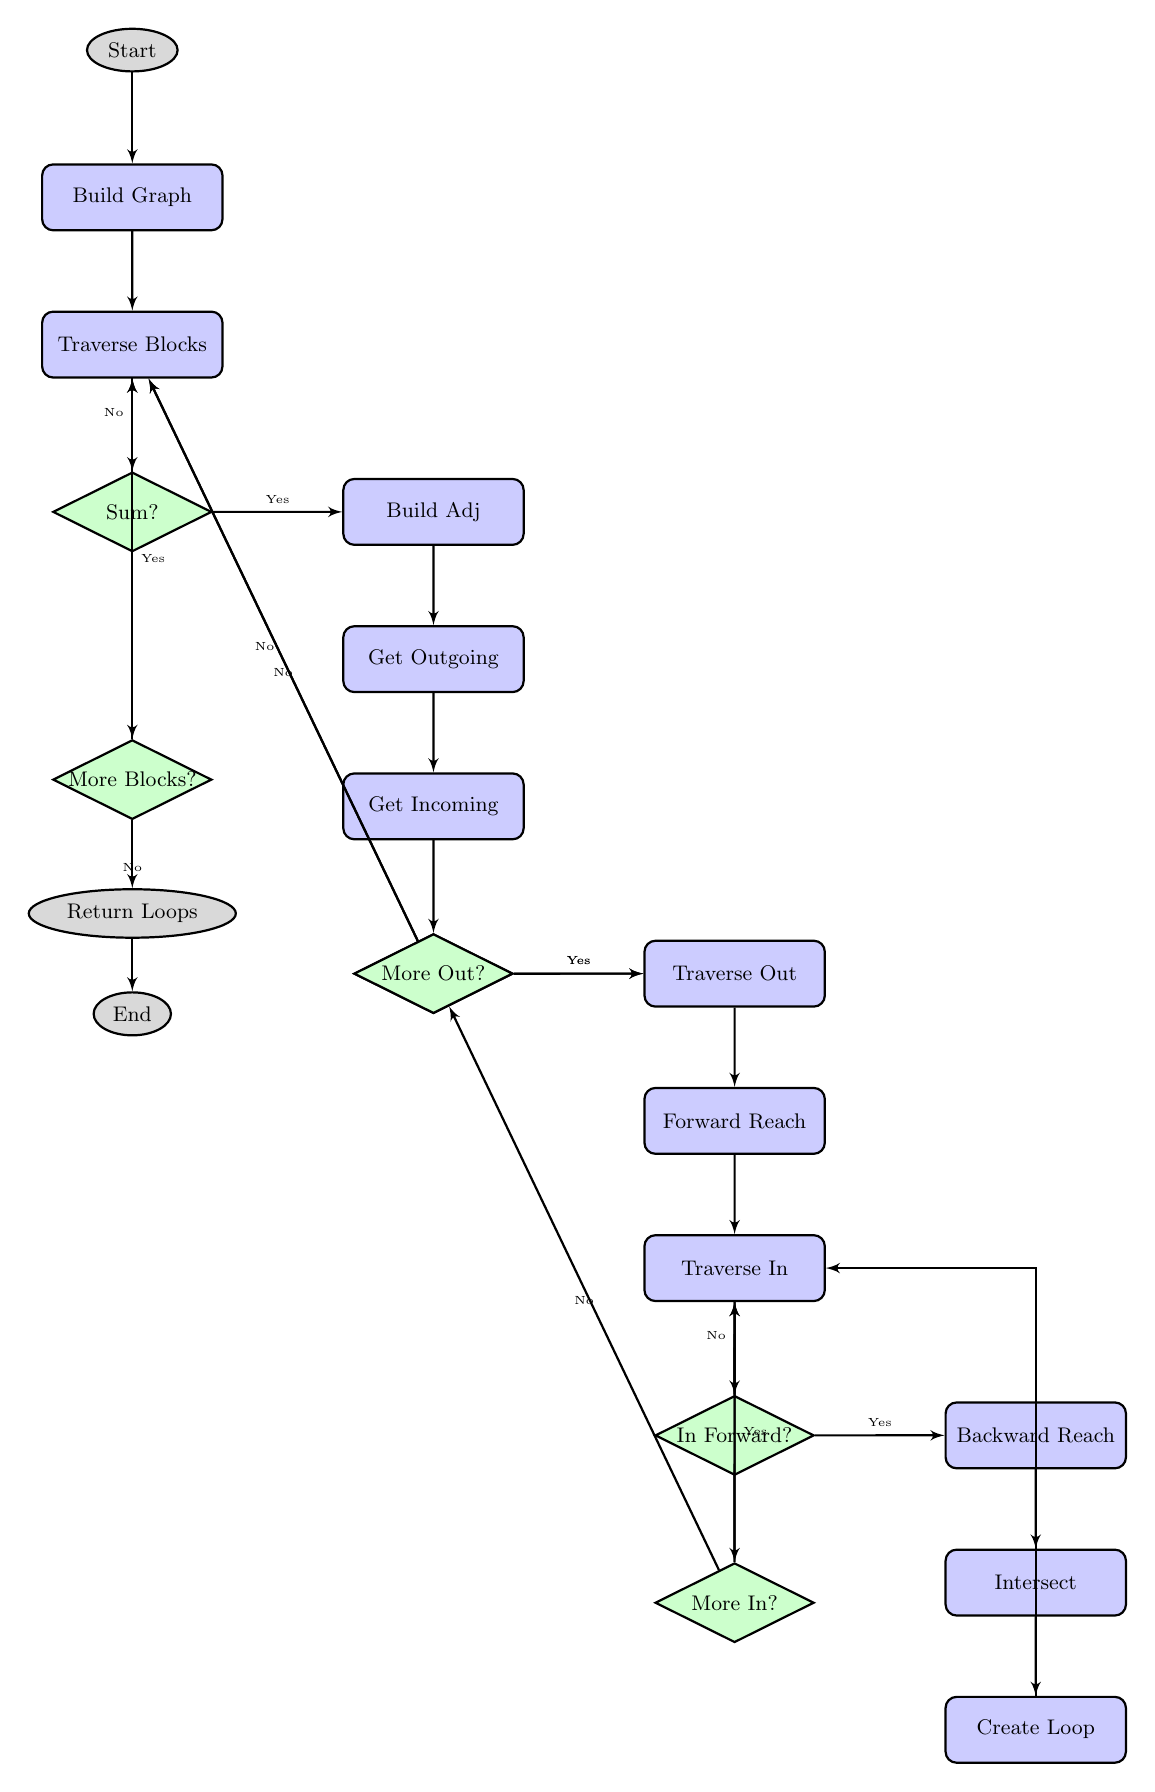
\begin{tikzpicture}[node distance=2.2cm, auto, scale=0.85, transform shape]
    \node [startstop] (start) {Start};
    \node [block, below of=start] (build) {Build Graph};
    \node [block, below of=build] (traverse) {Traverse Blocks};
    \node [decision, below of=traverse, node distance=2.5cm] (issum) {Sum?};
    \node [block, right of=issum, node distance=4.5cm] (buildadj) {Build Adj};
    \node [block, below of=buildadj] (getout) {Get Outgoing};
    \node [block, below of=getout] (getin) {Get Incoming};
    \node [decision, below of=getin, node distance=2.5cm] (hasboth) {Both?};
    \node [block, right of=hasboth, node distance=4.5cm] (traverseout) {Traverse Out};
    \node [block, below of=traverseout] (forward) {Forward Reach};
    \node [block, below of=forward] (traversein) {Traverse In};
    \node [decision, below of=traversein, node distance=2.5cm] (inforward) {In Forward?};
    \node [block, right of=inforward, node distance=4.5cm] (backward) {Backward Reach};
    \node [block, below of=backward] (intersect) {Intersect};
    \node [block, below of=intersect] (create) {Create Loop};
    \node [decision, below of=traversein, node distance=5cm] (morein) {More In?};
    \node [decision, left of=traverseout, node distance=4.5cm] (moreout) {More Out?};
    \node [decision, below of=traverse, node distance=6.5cm] (moreblocks) {More Blocks?};
    \node [startstop, below of=moreblocks, node distance=2cm] (return) {Return Loops};
    \node [startstop, below of=return, node distance=1.5cm] (end) {End};

    \path [line] (start) -- (build);
    \path [line] (build) -- (traverse);
    \path [line] (traverse) -- (issum);
    \path [line] (issum) -- node [above left, font=\tiny] {No} (traverse);
    \path [line] (issum) -- node [above, font=\tiny] {Yes} (buildadj);
    \path [line] (buildadj) -- (getout);
    \path [line] (getout) -- (getin);
    \path [line] (getin) -- (hasboth);
    \path [line] (hasboth) -- node [above left, font=\tiny] {No} (traverse);
    \path [line] (hasboth) -- node [above, font=\tiny] {Yes} (traverseout);
    \path [line] (traverseout) -- (forward);
    \path [line] (forward) -- (traversein);
    \path [line] (traversein) -- (inforward);
    \path [line] (inforward) -- node [above left, font=\tiny] {No} (traversein);
    \path [line] (inforward) -- node [above, font=\tiny] {Yes} (backward);
    \path [line] (backward) -- (intersect);
    \path [line] (intersect) -- (create);
    \path [line] (create) |- (traversein);
    \path [line] (traversein) -- (morein);
    \path [line] (morein) -- node [right, font=\tiny] {Yes} (traversein);
    \path [line] (morein) -- node [below, font=\tiny] {No} (moreout);
    \path [line] (moreout) -- node [above, font=\tiny] {Yes} (traverseout);
    \path [line] (moreout) -- node [below, font=\tiny] {No} (traverse);
    \path [line] (traverse) -- (moreblocks);
    \path [line] (moreblocks) -- node [right, font=\tiny] {Yes} (traverse);
    \path [line] (moreblocks) -- node [below, font=\tiny] {No} (return);
    \path [line] (return) -- (end);
\end{tikzpicture}
\caption{Loop Detection Algorithm Flowchart}
\label{fig:loopdetection}
\end{figure}

\subsection{Algorithm Steps}

\subsubsection{Data Structure Construction}

Convert control system blocks to graph nodes and connections to directed edges:

\begin{lstlisting}[language=JavaScript, caption=Data Structure Construction]
const blocks = Array.from(state.blocks.values()).map((block) => ({
  id: block.id,
  type: block.type,
  params: block.params || {},
}));

const connections = state.connections.map((conn) => ({
  from: conn.from,
  to: conn.to,
  fromIndex: conn.fromIndex ?? 0,
  toIndex: conn.toIndex ?? 0,
}));
\end{lstlisting}

\subsubsection{Graph Traversal Function}

Use Depth-First Search (DFS) to traverse the graph:

\begin{lstlisting}[language=JavaScript, caption=Graph Traversal Function]
const traverse = (startId, adj, sumId) => {
  const visited = new Set();
  const stack = [startId];
  while (stack.length) {
    const id = stack.pop();
    if (visited.has(id)) continue;
    visited.add(id);
    (adj.get(id) || []).forEach((next) => {
      if (next === sumId) return;
      stack.push(next);
    });
  }
  return visited;
};
\end{lstlisting}

\textbf{Time Complexity}: O(V + E), where V is the number of nodes and E is the number of edges.

\subsubsection{Loop Detection Main Logic}

\textbf{1. Filter Sum Blocks}

\begin{lstlisting}[language=JavaScript]
const loops = [];
blocks.forEach((block) => {
  if (block.type !== "sum") return;
  const sumId = block.id;
  // ... subsequent processing
});
\end{lstlisting}

\textbf{2. Build Adjacency List}

\begin{lstlisting}[language=JavaScript, caption=Build Adjacency List]
const signs = Array.isArray(block.params?.signs) ? block.params.signs : [];
const forward = new Map();
const backward = new Map();

blocks.forEach((node) => {
  forward.set(node.id, []);
  backward.set(node.id, []);
});

connections.forEach((conn) => {
  if (!forward.has(conn.from) || !forward.has(conn.to)) return;
  if (conn.from === sumId || conn.to === sumId) return;
  forward.get(conn.from).push(conn.to);
  backward.get(conn.to).push(conn.from);
});
\end{lstlisting}

\textbf{3. Bidirectional Traversal to Determine Loops}

\begin{lstlisting}[language=JavaScript, caption=Bidirectional Traversal]
const outgoing = connections.filter((conn) => conn.from === sumId);
const incoming = connections.filter((conn) => conn.to === sumId);

if (!outgoing.length || !incoming.length) return;

outgoing.forEach((outConn) => {
  const forwardReach = traverse(outConn.to, forward, sumId);
  
  incoming.forEach((inConn) => {
    if (!forwardReach.has(inConn.from)) return;
    
    const backwardReach = traverse(inConn.from, backward, sumId);
    
    const activeIds = new Set(
      Array.from(forwardReach).filter((id) => backwardReach.has(id))
    );
    
    activeIds.add(outConn.to);
    activeIds.add(inConn.from);
    activeIds.delete(sumId);
    
    const feedbackSign = Number(signs[inConn.toIndex ?? 0] ?? 1) || 0;
    
    const key = `${sumId}:${outConn.to}:${outConn.fromIndex ?? 0}->${inConn.from}:${inConn.toIndex ?? 0}`;
    loops.push({
      key,
      sumId,
      outConn,
      inConn,
      activeIds,
      feedbackSign,
    });
  });
});
\end{lstlisting}

\subsection{Algorithm Complexity Analysis}

\subsubsection{Time Complexity}

\begin{itemize}
    \item Build adjacency list: O(V + E)
    \item Traverse sum blocks: O(V)
    \item Processing each sum block:
    \begin{itemize}
        \item Forward traversal: O(V + E)
        \item Backward traversal: O(V + E)
        \item Intersection calculation: O(V)
    \end{itemize}
    \item \textbf{Total Complexity}: O(n × (V + E)), where n is the number of sum blocks
\end{itemize}

\subsubsection{Space Complexity}

\begin{itemize}
    \item Adjacency list storage: O(V + E)
    \item Reachable set storage: O(V)
    \item Loop storage: O(n × V)
    \item \textbf{Total Complexity}: O(V + E + n × V)
\end{itemize}

\subsection{Algorithm Characteristics}

\subsubsection{Advantages}

\begin{enumerate}
    \item \textbf{Precise loop localization}: Not only know loop exists but also identify specific nodes
    \item \textbf{Multi-loop support}: Can detect all feedback loops in the system
    \item \textbf{Preserve loop information}: Record input/output connections and feedback signs
    \item \textbf{Control system oriented}: Specifically designed for control system feedback structures
    \item \textbf{High efficiency}: Very efficient for sparse graphs
\end{enumerate}

\subsubsection{Limitations}

\begin{enumerate}
    \item \textbf{Depends on sum blocks}: Only detects loops formed through sum blocks
    \item \textbf{No algebraic loop handling}: Does not detect algebraic loops not involving sum blocks
    \item \textbf{Assumes directed graph}: Assumes control system is a directed graph, does not handle bidirectional connections
\end{enumerate}

\subsection{Comparison with Other Algorithms}

\begin{table}[H]
\centering
\caption{Comparison with Kahn's Algorithm}
\begin{tabular}{lll}
\toprule
\textbf{Feature} & \textbf{Kahn's Algorithm} & \textbf{Vibesim Algorithm} \\
\midrule
Main Purpose & Topological Sort & Loop Detection and Localization \\
Detection Method & Remove nodes with indegree 0 & Bidirectional Traversal Intersection \\
Loop Information & Only know existence & Precise localization of composition \\
Time Complexity & O(V+E) & O(n×(V+E)) \\
Applicable Scenario & Directed Acyclic Graph & Control System Feedback Loop \\
\bottomrule
\end{tabular}
\end{table}

\begin{table}[H]
\centering
\caption{Comparison with Standard DFS Loop Detection}
\begin{tabular}{lll}
\toprule
\textbf{Feature} & \textbf{Standard DFS} & \textbf{Vibesim Algorithm} \\
\midrule
Detection Method & Recursive stack detection & Bidirectional Traversal Intersection \\
Loop Information & Stop when found & Complete traversal of all loops \\
System Specificity & General graph algorithm & Control system specific \\
Feedback Sign & Not handled & Record feedback sign \\
\bottomrule
\end{tabular}
\end{table}

\subsection{Example Analysis}

\subsubsection{Simple Feedback System}

\begin{figure}[H]
\centering
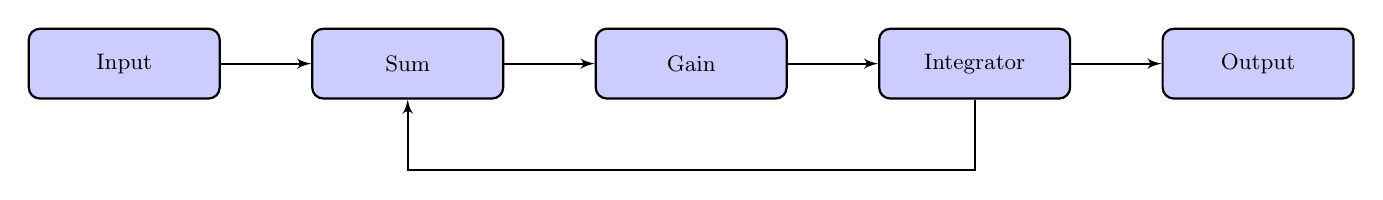
\begin{tikzpicture}[node distance=3cm, auto, scale=0.9, transform shape]
    \node [block] (input) {Input};
    \node [block, right of=input, node distance=4cm] (sum) {Sum};
    \node [block, right of=sum, node distance=4cm] (gain) {Gain};
    \node [block, right of=gain, node distance=4cm] (int) {Integrator};
    \node [block, right of=int, node distance=4cm] (output) {Output};

    \path [line] (input) -- (sum);
    \path [line] (sum) -- (gain);
    \path [line] (gain) -- (int);
    \path [line] (int) -- (output);
    \path [line] (int.south) -- ++(0,-1) -| (sum.south);
\end{tikzpicture}
\caption{Simple Feedback System}
\label{fig:simplefeedback}
\end{figure}

\textbf{Algorithm Execution Process}:
\begin{enumerate}
    \item Identify sum block
    \item Outgoing connection: Sum → Gain
    \item Incoming connection: Integrator → Sum
    \item Forward traversal: \{Gain, Integrator\}
    \item Backward traversal: \{Integrator, Gain\}
    \item Intersection: \{Gain, Integrator\}
    \item Loop detected
\end{enumerate}

\newpage

\section{Solver Details}

\subsection{Overview}

Vibesim solver is responsible for numerical simulation of control systems, including integration calculation, algorithm selection, and loop convergence handling. The solver uses a phased processing approach to ensure numerical accuracy and efficiency.

\subsection{Integration Processing}

\subsubsection{Main Integration Algorithm: RK4 (Fourth-Order Runge-Kutta)}

Vibesim primarily uses the RK4 algorithm for numerical integration, which is one of the most commonly used numerical integration methods with high accuracy and good stability.

\paragraph{Basic RK4 Implementation}

\begin{lstlisting}[language=JavaScript, caption=Basic RK4 Implementation]
export const integrateRK4 = (state, input, dt) => {
  const k1 = input;
  const k2 = input;
  const k3 = input;
  const k4 = input;
  return state + (dt / 6) * (k1 + 2 * k2 + 2 * k3 + k4);
};
\end{lstlisting}

\textbf{Description}:
\begin{itemize}
    \item For pure integrators (input directly as derivative), RK4 simplifies to the above form
    \item \texttt{state}: Current state value
    \item \texttt{input}: Input value (i.e., derivative)
    \item \texttt{dt}: Time step
    \item Returns: Next time step state value
\end{itemize}

\paragraph{Transfer Function RK4 Implementation}

\begin{lstlisting}[language=JavaScript, caption=Transfer Function RK4 Implementation]
export const integrateTfRK4 = (model, state, input, dt) => {
  if (model.n === 0) return state;
  const k1 = stateDerivative(model, state, input);
  const k2 = stateDerivative(model, addVec(state, scaleVec(k1, dt / 2)), input);
  const k3 = stateDerivative(model, addVec(state, scaleVec(k2, dt / 2)), input);
  const k4 = stateDerivative(model, addVec(state, scaleVec(k3, dt)), input);
  const sum = addVec(addVec(k1, scaleVec(k2, 2)), addVec(scaleVec(k3, 2), k4));
  return addVec(state, scaleVec(sum, dt / 6));
};
\end{lstlisting}

\textbf{Description}:
\begin{itemize}
    \item \texttt{model}: State space model of transfer function
    \item \texttt{state}: Current state vector
    \item \texttt{input}: Input value
    \item \texttt{dt}: Time step
    \item Uses complete RK4 four-step calculation
\end{itemize}

\subsubsection{Integrator Block Implementation}

The integrator block is the most basic continuous-time block in control systems, implemented as follows:

\begin{lstlisting}[language=JavaScript, caption=Integrator Block Implementation]
integrator: {
  init: (ctx, block) => {
    const params = ctx.resolvedParams.get(block.id) || {};
    const state = getBlockState(ctx, block);
    const min = resolveLimit(params.min, -Infinity);
    const max = resolveLimit(params.max, Infinity);
    const initial = Number(params.initial) || 0;
    state.integrator = clampValue(initial, min, max);
  },
  output: (ctx, block) => {
    const state = getBlockState(ctx, block);
    const prev = state.integrator ?? 0;
    ctx.outputs.set(block.id, prev);
  },
  update: (ctx, block) => {
    const params = ctx.resolvedParams.get(block.id) || {};
    const min = resolveLimit(params.min, -Infinity);
    const max = resolveLimit(params.max, Infinity);
    const inputVal = getInputValue(ctx, block, 0, 0);
    const state = getBlockState(ctx, block);
    const prev = state.integrator ?? 0;
    const next = integrateRK4(prev, inputVal ?? 0, ctx.dt);
    state.integrator = clampValue(next, min, max);
  },
}
\end{lstlisting}

\textbf{Features}:
\begin{enumerate}
    \item \textbf{Clamping support}: Can set minimum and maximum values for integrator
    \item \textbf{Initial conditions}: Supports setting initial values for integrator
    \item \textbf{Three-phase processing}:
    \begin{itemize}
        \item \texttt{init}: Initialize state
        \item \texttt{output}: Output current state
        \item \texttt{update}: Update state using RK4
    \end{itemize}
\end{enumerate}

\subsubsection{RK4 Algorithm Advantages}

\begin{table}[H]
\centering
\caption{RK4 Algorithm Advantages}
\begin{tabular}{ll}
\toprule
\textbf{Feature} & \textbf{Description} \\
\midrule
High Accuracy & Fourth-order accuracy, error is O(dt$^5$) \\
Stability & Good stability for most systems \\
Efficiency & Requires 4 derivative calculations per step \\
Widely Used & Most commonly used numerical integration method in engineering \\
\bottomrule
\end{tabular}
\end{table}

\subsection{Algorithm Selection Strategy}

\subsubsection{Fixed Algorithm Strategy}

Vibesim \textbf{does not provide user-selectable integration algorithms}, but instead uses a fixed algorithm strategy based on block types. This design simplifies user operations while ensuring sufficient numerical accuracy.

\subsubsection{Continuous-Time System Algorithms}

\paragraph{Integrator}
\begin{itemize}
    \item \textbf{Algorithm}: Simplified RK4
    \item \textbf{Reason}: Pure integrator, derivative directly equals input
    \item \textbf{Code}: \texttt{integrateRK4}
\end{itemize}

\paragraph{Transfer Function}
\begin{itemize}
    \item \textbf{Algorithm}: Complete RK4 (state space form)
    \item \textbf{Reason}: Need to handle state vectors and matrix operations
    \item \textbf{Code}: \texttt{integrateTfRK4}
\end{itemize}

\paragraph{State Space}
\begin{itemize}
    \item \textbf{Algorithm}: Forward Euler
    \item \textbf{Reason}: Simple first-order system
\end{itemize}

\begin{lstlisting}[language=JavaScript]
const xNext = prev + ctx.dt * (A * prev + B * (inputVal ?? 0));
state.stateSpaceX = xNext;
const y = C * xNext + D * (inputVal ?? 0);
\end{lstlisting}

\paragraph{PID Controller}
\begin{itemize}
    \item \textbf{Algorithm}: Forward Euler (integral part)
    \item \textbf{Reason}: Simple method sufficient for integral term
\end{itemize}

\begin{lstlisting}[language=JavaScript]
const nextIntegral = pid.integral + (inputVal ?? 0) * ctx.dt;
const clampedIntegral = clampValue(nextIntegral, min, max);
const derivative = ((inputVal ?? 0) - pid.prev) / Math.max(ctx.dt, 1e-6);
const out = kp * (inputVal ?? 0) + ki * clampedIntegral + kd * derivative;
\end{lstlisting}

\paragraph{Low/High Pass Filter (LPF/HPF)}
\begin{itemize}
    \item \textbf{Algorithm}: Forward Euler
    \item \textbf{Reason}: First-order filter, simple method sufficient
\end{itemize}

\begin{lstlisting}[language=JavaScript]
const wc = 2 * Math.PI * fc;
const next = prev + ctx.dt * wc * ((inputVal ?? 0) - prev);
\end{lstlisting}

\paragraph{Derivative}
\begin{itemize}
    \item \textbf{Algorithm}: Finite Difference
    \item \textbf{Reason}: Derivative requires discretization
\end{itemize}

\begin{lstlisting}[language=JavaScript]
const out = ((inputVal ?? 0) - prev) / Math.max(ctx.dt, 1e-6);
\end{lstlisting}

\subsubsection{Discrete-Time System Algorithms}

\paragraph{Zero-Order Hold (ZOH)}
\begin{itemize}
    \item \textbf{Algorithm}: Piecewise constant
    \item \textbf{Feature}: Holds last sampled value during sampling interval
\end{itemize}

\begin{lstlisting}[language=JavaScript]
if (ctx.t + 1e-6 >= state.nextTime) {
  state.lastSample = inputVal ?? 0;
  state.nextTime = ctx.t + ts;
}
\end{lstlisting}

\paragraph{First-Order Hold (FOH)}
\begin{itemize}
    \item \textbf{Algorithm}: Linear interpolation
    \item \textbf{Feature}: Linear interpolation during sampling interval
\end{itemize}

\begin{lstlisting}[language=JavaScript]
const slope = (state.lastSample - state.prevSample) / ts;
const out = state.lastSample + slope * (ctx.t - state.lastTime);
\end{lstlisting}

\paragraph{Discrete Transfer Function (DTF)}
\begin{itemize}
    \item \textbf{Algorithm}: Difference equation
    \item \textbf{Feature}: Uses input and output history values
\end{itemize}

\begin{lstlisting}[language=JavaScript]
let y = 0;
for (let i = 0; i < num.length; i += 1) {
  y += (num[i] || 0) * (xHist[i] || 0);
}
for (let i = 1; i < den.length; i += 1) {
  y -= (den[i] || 0) * (yHist[i - 1] || 0);
}
\end{lstlisting}

\paragraph{Discrete Delay (DDelay)}
\begin{itemize}
    \item \textbf{Algorithm}: Queue implementation
    \item \textbf{Feature}: Uses queue to store history values
\end{itemize}

\begin{lstlisting}[language=JavaScript]
state.queue.push(inputVal ?? 0);
while (state.queue.length > steps) state.queue.shift();
state.lastOut = state.queue[0] ?? 0;
\end{lstlisting}

\subsubsection{Algorithm Selection Flowchart}

\begin{figure}[H]
\centering
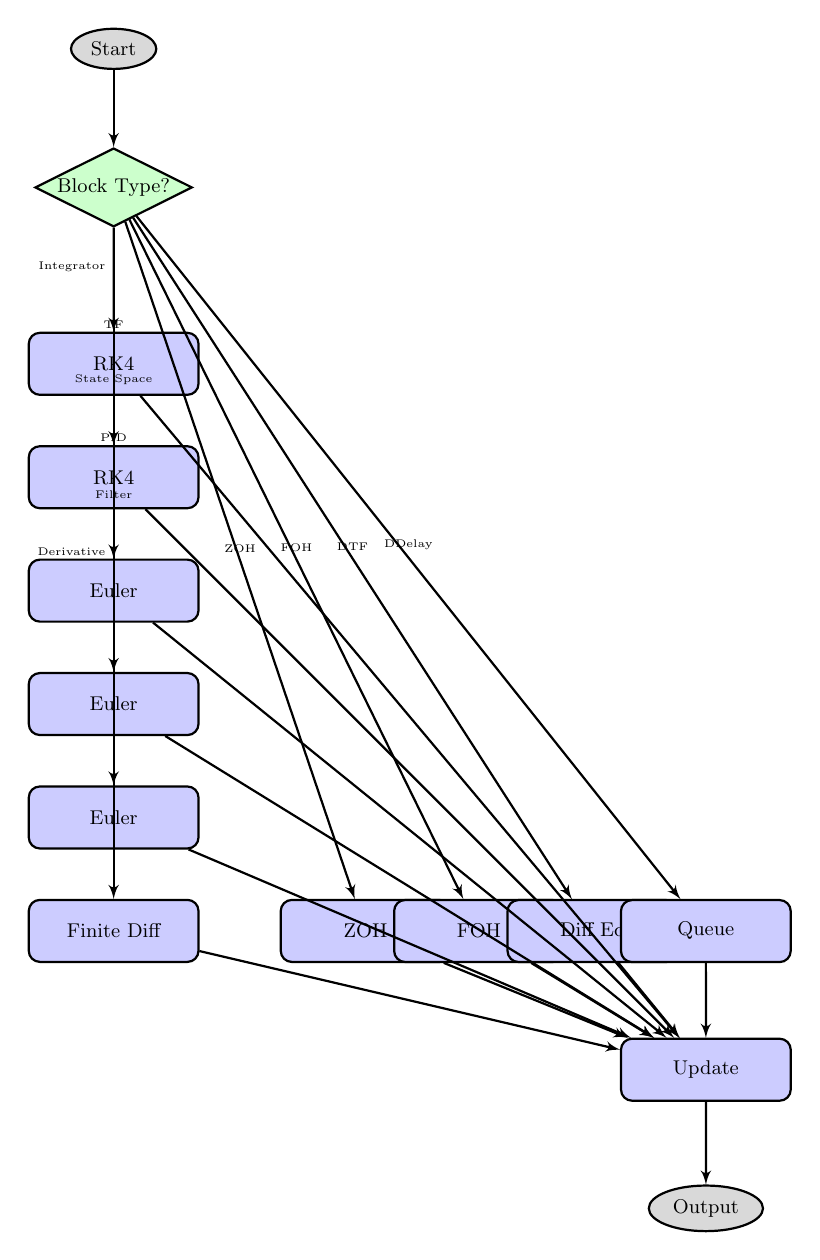
\begin{tikzpicture}[node distance=1.8cm, auto, scale=0.8, transform shape]
    \node [startstop] (start) {Start};
    \node [decision, below of=start, node distance=2.2cm] (type) {Block Type?};
    \node [block, below of=type, node distance=2.8cm] (integrator) {RK4};
    \node [block, below of=integrator] (tf) {RK4};
    \node [block, below of=tf] (statespace) {Euler};
    \node [block, below of=statespace] (pid) {Euler};
    \node [block, below of=pid] (filter) {Euler};
    \node [block, below of=filter] (derivative) {Finite Diff};
    \node [block, right of=derivative, node distance=4cm] (zoh) {ZOH};
    \node [block, right of=zoh] (foh) {FOH};
    \node [block, right of=foh] (dtf) {Diff Eq};
    \node [block, right of=dtf] (ddelay) {Queue};
    \node [block, below of=ddelay, node distance=2.2cm] (update) {Update};
    \node [startstop, below of=update, node distance=2.2cm] (output) {Output};

    \path [line] (start) -- (type);
    \path [line] (type) -- node [above left, font=\tiny] {Integrator} (integrator);
    \path [line] (type) -- node [above, font=\tiny] {TF} (tf);
    \path [line] (type) -- node [above, font=\tiny] {State Space} (statespace);
    \path [line] (type) -- node [above, font=\tiny] {PID} (pid);
    \path [line] (type) -- node [above, font=\tiny] {Filter} (filter);
    \path [line] (type) -- node [above left, font=\tiny] {Derivative} (derivative);
    \path [line] (type) -- node [above, font=\tiny] {ZOH} (zoh);
    \path [line] (type) -- node [above, font=\tiny] {FOH} (foh);
    \path [line] (type) -- node [above, font=\tiny] {DTF} (dtf);
    \path [line] (type) -- node [above, font=\tiny] {DDelay} (ddelay);
    \path [line] (integrator) -- (update);
    \path [line] (tf) -- (update);
    \path [line] (statespace) -- (update);
    \path [line] (pid) -- (update);
    \path [line] (filter) -- (update);
    \path [line] (derivative) -- (update);
    \path [line] (zoh) -- (update);
    \path [line] (foh) -- (update);
    \path [line] (dtf) -- (update);
    \path [line] (ddelay) -- (update);
    \path [line] (update) -- (output);
\end{tikzpicture}
\caption{Algorithm Selection Flowchart}
\label{fig:algorithmselection}
\end{figure}

\subsubsection{Algorithm Selection Summary Table}

\begin{table}[H]
\centering
\caption{Algorithm Selection Summary}
\begin{tabular}{llll}
\toprule
\textbf{Block Type} & \textbf{Algorithm} & \textbf{Accuracy} & \textbf{Use Case} \\
\midrule
Integrator & RK4 & O(dt$^5$) & Continuous-time integration \\
Transfer Function & RK4 & O(dt$^5$) & Continuous-time dynamics \\
State Space & Forward Euler & O(dt$^2$) & First-order system \\
PID & Forward Euler & O(dt$^2$) & Controller \\
LPF/HPF & Forward Euler & O(dt$^2$) & Filter \\
Derivative & Finite Difference & O(dt) & Derivative calculation \\
ZOH & Piecewise Constant & Exact & Discrete hold \\
FOH & Linear Interpolation & Exact & Discrete hold \\
DTF & Difference Equation & Exact & Discrete transfer function \\
DDelay & Queue & Exact & Discrete delay \\
\bottomrule
\end{tabular}
\end{table}

\subsection{Loop Convergence Processing}

\subsubsection{Algebraic Loop Concept}

Algebraic loops refer to pure algebraic dependency loops that do not involve integrators or delays, for example:

\begin{figure}[H]
\centering
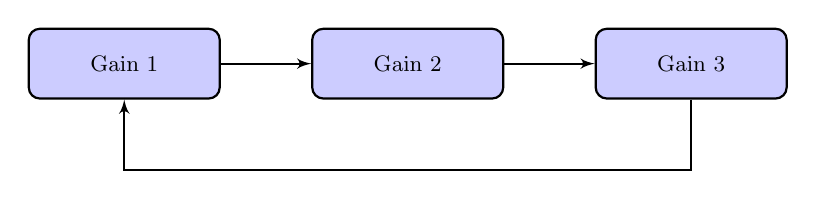
\begin{tikzpicture}[node distance=3cm, auto, scale=0.9, transform shape]
    \node [block] (gain1) {Gain 1};
    \node [block, right of=gain1, node distance=4cm] (gain2) {Gain 2};
    \node [block, right of=gain2, node distance=4cm] (gain3) {Gain 3};

    \path [line] (gain1) -- (gain2);
    \path [line] (gain2) -- (gain3);
    \path [line] (gain3.south) -- ++(0,-1) -| (gain1.south);
\end{tikzpicture}
\caption{Algebraic Loop Example}
\label{fig:algebraicloop}
\end{figure}

Such loops cannot be solved through time progression and require special convergence algorithms.

\subsubsection{Algebraic Loop Detection}

\paragraph{Topological Sort (Kahn's Algorithm)}

\begin{lstlisting}[language=JavaScript, caption=Topological Sort]
function buildAlgebraicPlan(algebraicBlocks, inputMap) {
  const byId = new Map();
  algebraicBlocks.forEach((entry) => byId.set(entry.block.id, entry));
  if (byId.size === 0) return { ordered: [], hasCycle: false };

  const indegree = new Map();
  const outEdges = new Map();
  byId.forEach((_, id) => {
    indegree.set(id, 0);
    outEdges.set(id, new Set());
  });

  byId.forEach((_, targetId) => {
    const inputs = inputMap.get(targetId) || [];
    inputs.forEach((srcKey) => {
      const srcId = sourceBlockIdFromKey(srcKey);
      if (!srcId || !byId.has(srcId) || srcId === targetId) return;
      const edges = outEdges.get(srcId);
      if (edges.has(targetId)) return;
      edges.add(targetId);
      indegree.set(targetId, (indegree.get(targetId) || 0) + 1);
    });
  });

  const queue = [];
  indegree.forEach((deg, id) => {
    if (deg === 0) queue.push(id);
  });
  const ordered = [];
  let readIdx = 0;
  while (readIdx < queue.length) {
    const id = queue[readIdx];
    readIdx += 1;
    ordered.push(byId.get(id));
    outEdges.get(id).forEach((neighbor) => {
      const next = (indegree.get(neighbor) || 0) - 1;
      indegree.set(neighbor, next);
      if (next === 0) queue.push(neighbor);
    });
  }

  const hasCycle = ordered.length !== byId.size;
  return { ordered: hasCycle ? algebraicBlocks : ordered, hasCycle };
}
\end{lstlisting}

\textbf{Description}:
\begin{itemize}
    \item If topological sort succeeds (\texttt{ordered.length === byId.size}), there is no loop
    \item If topological sort fails, an algebraic loop exists
    \item Returns sorted block list and loop flag
\end{itemize}

\subsubsection{Algebraic Loop Convergence Algorithm}

\paragraph{Fixed-Point Iteration}

\begin{lstlisting}[language=JavaScript, caption=Fixed-Point Iteration]
if (run.needsAlgebraicSolve) {
  if (!run.hasLabelResolution && !run.algebraicPlan.hasCycle) {
    run.algebraicPlan.ordered.forEach(({ block, handler }) => {
      handler.algebraic(run.ctx, block);
    });
  } else {
    let progress = true;
    let iter = 0;
    const maxIter = 50;
    while (progress && iter < maxIter) {
      iter += 1;
      progress = false;
      
      if (run.hasLabelResolution && resolveLabelSources()) 
        progress = true;
      
      run.algebraicPlan.ordered.forEach(({ block, handler }) => {
        const result = handler.algebraic(run.ctx, block);
        if (result?.updated) progress = true;
      });
      
      if (run.hasLabelResolution && resolveLabelSources()) 
        progress = true;
    }
    
    if (progress && iter >= maxIter) {
      run.algebraicLoopFailed = true;
      run.algebraicLoopTime = t;
      return false;
    }
  }
}
\end{lstlisting}

\textbf{Convergence Conditions}:
\begin{itemize}
    \item All algebraic block values no longer change
    \item Or reach maximum iteration count (50 times)
\end{itemize}

\subsubsection{Algebraic Block Processing Example}

\paragraph{Transfer Function (Zero-Order)}

\begin{lstlisting}[language=JavaScript, caption=Transfer Function Algebraic Processing]
algebraic: (ctx, block) => {
  const state = getBlockState(ctx, block);
  const model = state.tfModel;
  if (!model || model.n !== 0) return null;
  const inputVal = getInputValue(ctx, block, 0, 0);
  const out = outputFromState(model, model.state || [], inputVal ?? 0);
  const prev = ctx.outputs.get(block.id);
  ctx.outputs.set(block.id, out);
  return { updated: prev !== out && !(Number.isNaN(prev) && Number.isNaN(out)) };
}
\end{lstlisting}

\textbf{Description}:
\begin{itemize}
    \item For zero-order transfer functions (pure gain), use algebraic processing
    \item Returns flag indicating whether value was updated
    \item Used for detecting convergence state
\end{itemize}

\subsubsection{Loop Convergence Flowchart}

\begin{figure}[H]
\centering
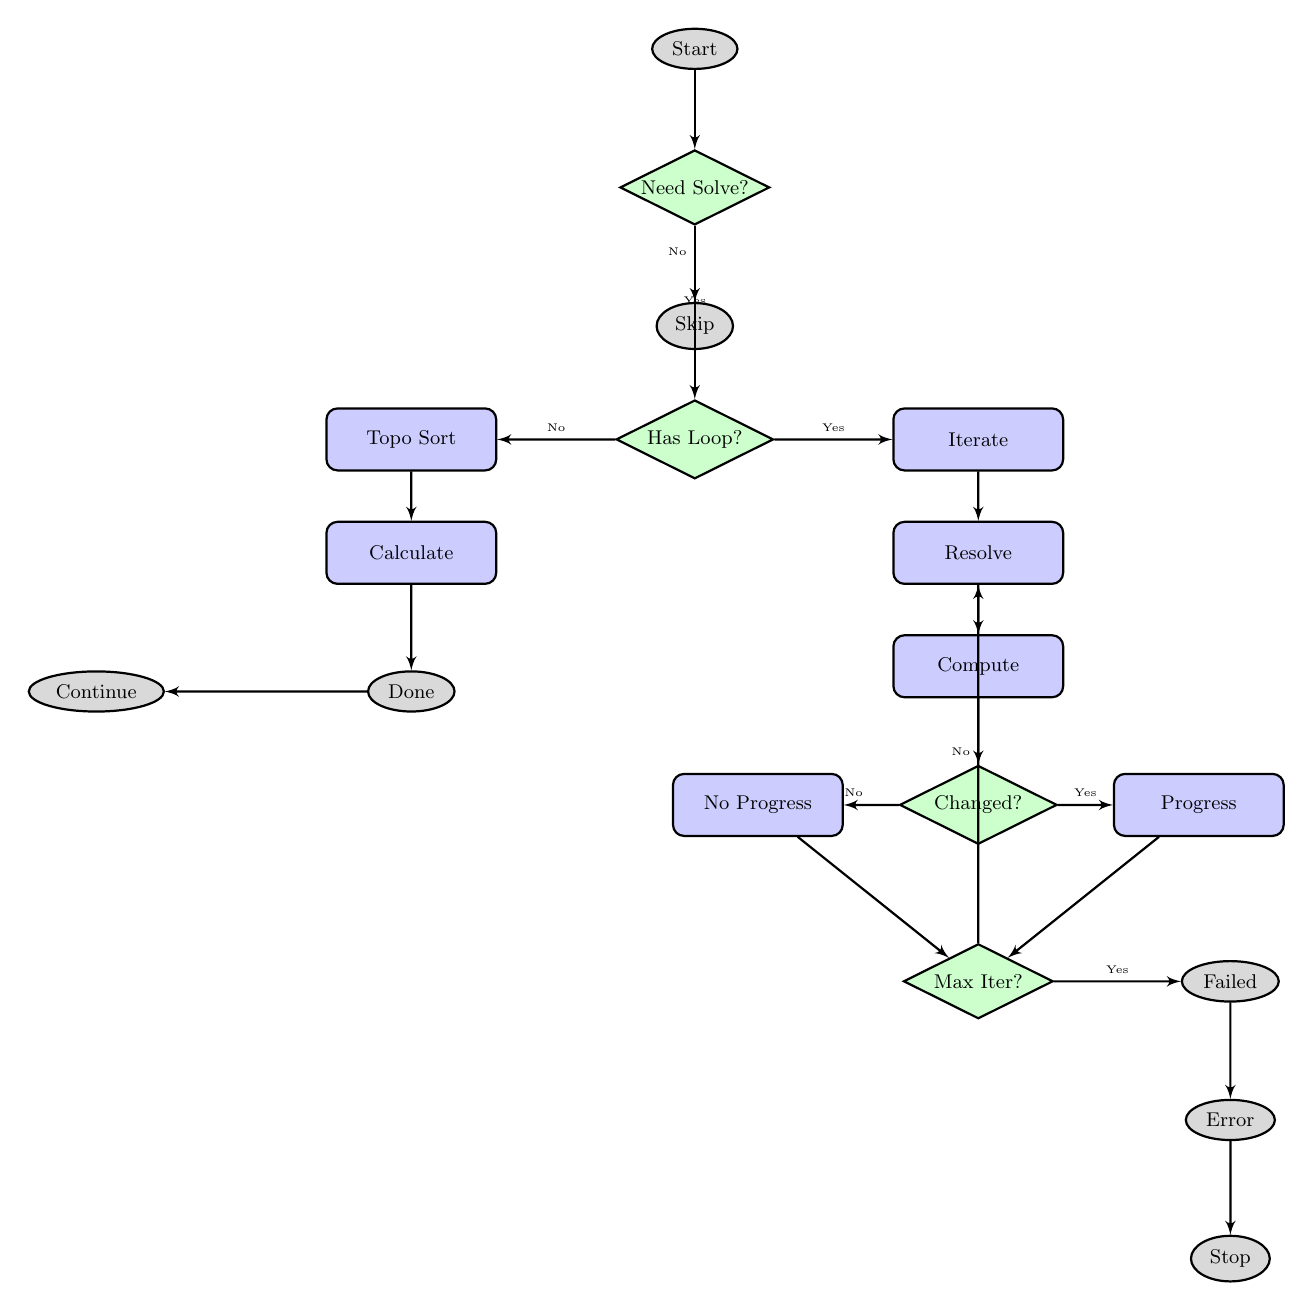
\begin{tikzpicture}[node distance=1.8cm, auto, scale=0.8, transform shape]
    \node [startstop] (start) {Start};
    \node [decision, below of=start, node distance=2.2cm] (need) {Need Solve?};
    \node [startstop, below of=need, node distance=2.2cm] (skip) {Skip};
    \node [decision, below of=need, node distance=4cm] (hascycle) {Has Loop?};
    \node [block, left of=hascycle, node distance=4.5cm] (topo) {Topo Sort};
    \node [block, below of=topo] (calc) {Calculate};
    \node [startstop, below of=calc, node distance=2.2cm] (done) {Done};
    \node [block, right of=hascycle, node distance=4.5cm] (iterate) {Iterate};
    \node [block, below of=iterate] (resolve) {Resolve};
    \node [block, below of=resolve] (compute) {Compute};
    \node [decision, below of=compute, node distance=2.2cm] (changed) {Changed?};
    \node [block, right of=changed, node distance=3.5cm] (progresstrue) {Progress};
    \node [block, left of=changed, node distance=3.5cm] (progressfalse) {No Progress};
    \node [decision, below of=changed, node distance=2.8cm] (maxiter) {Max Iter?};
    \node [startstop, right of=maxiter, node distance=4cm] (failed) {Failed};
    \node [startstop, below of=failed, node distance=2.2cm] (error) {Error};
    \node [startstop, below of=error, node distance=2.2cm] (stop) {Stop};
    \node [startstop, left of=done, node distance=5cm] (continue) {Continue};

    \path [line] (start) -- (need);
    \path [line] (need) -- node [above left, font=\tiny] {No} (skip);
    \path [line] (need) -- node [above, font=\tiny] {Yes} (hascycle);
    \path [line] (hascycle) -- node [above, font=\tiny] {No} (topo);
    \path [line] (topo) -- (calc);
    \path [line] (calc) -- (done);
    \path [line] (hascycle) -- node [above, font=\tiny] {Yes} (iterate);
    \path [line] (iterate) -- (resolve);
    \path [line] (resolve) -- (compute);
    \path [line] (compute) -- (changed);
    \path [line] (changed) -- node [above, font=\tiny] {Yes} (progresstrue);
    \path [line] (changed) -- node [above left, font=\tiny] {No} (progressfalse);
    \path [line] (progresstrue) -- (maxiter);
    \path [line] (progressfalse) -- (maxiter);
    \path [line] (maxiter) -- node [above left, font=\tiny] {No} (resolve);
    \path [line] (maxiter) -- node [above, font=\tiny] {Yes} (failed);
    \path [line] (failed) -- (error);
    \path [line] (error) -- (stop);
    \path [line] (done) -- (continue);
\end{tikzpicture}
\caption{Loop Convergence Flowchart}
\label{fig:loopconvergence}
\end{figure}

\subsubsection{Loop Convergence Characteristics}

\begin{table}[H]
\centering
\caption{Loop Convergence Characteristics}
\begin{tabular}{ll}
\toprule
\textbf{Feature} & \textbf{Description} \\
\midrule
Iteration Method & Fixed-point iteration \\
Convergence Detection & Check if values are stable \\
Maximum Iterations & 50 times \\
No Loop Optimization & Use topological sort, single calculation \\
Loop Processing & Iterate until convergence or timeout \\
Error Handling & Report specific time point when not converged \\
Label Support & Support label connections between subsystems \\
\bottomrule
\end{tabular}
\end{table}

\subsection{Solver Flow}

\subsubsection{Complete Solver Flow}

\begin{figure}[H]
\centering
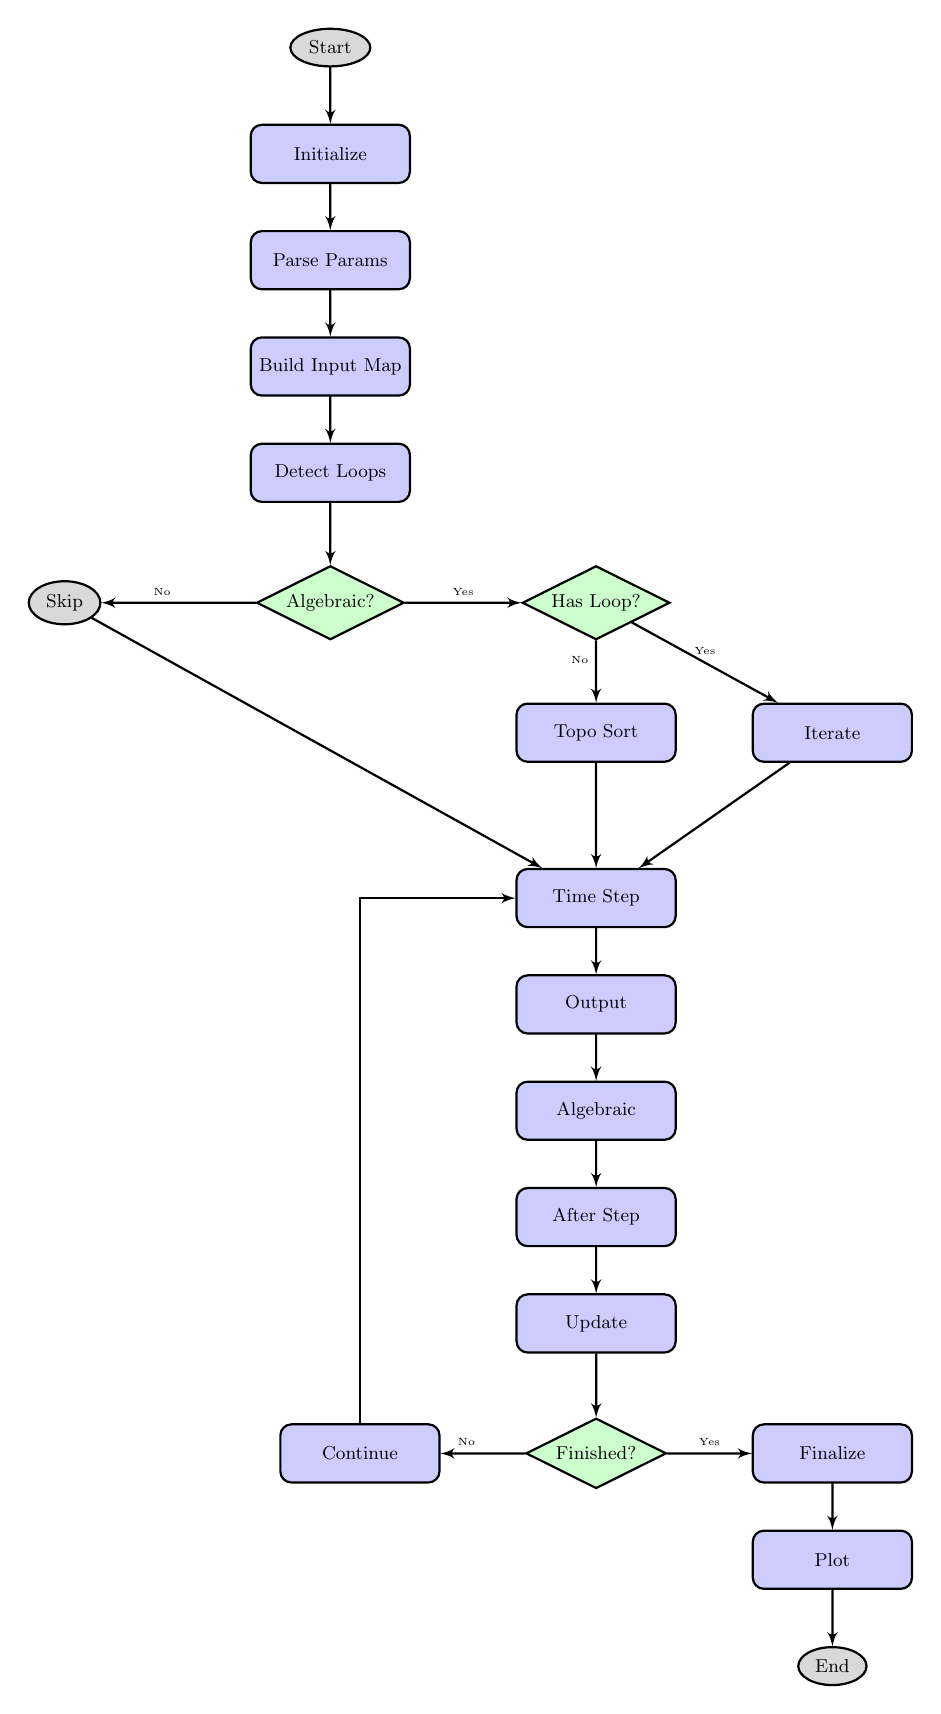
\begin{tikzpicture}[node distance=1.8cm, auto, scale=0.75, transform shape]
    \node [startstop] (start) {Start};
    \node [block, below of=start] (init) {Initialize};
    \node [block, below of=init] (parse) {Parse Params};
    \node [block, below of=parse] (build) {Build Input Map};
    \node [block, below of=build] (detect) {Detect Loops};
    \node [decision, below of=detect, node distance=2.2cm] (hasalgebraic) {Algebraic?};
    \node [startstop, left of=hasalgebraic, node distance=4.5cm] (skipalg) {Skip};
    \node [decision, right of=hasalgebraic, node distance=4.5cm] (hascycle) {Has Loop?};
    \node [block, below of=hascycle, node distance=2.2cm] (topo) {Topo Sort};
    \node [block, right of=topo, node distance=4cm] (iterate) {Iterate};
    \node [block, below of=topo, node distance=2.8cm] (step) {Time Step};
    \node [block, below of=step] (output) {Output};
    \node [block, below of=output] (algebraic) {Algebraic};
    \node [block, below of=algebraic] (afterstep) {After Step};
    \node [block, below of=afterstep] (update) {Update};
    \node [decision, below of=update, node distance=2.2cm] (finished) {Finished?};
    \node [block, left of=finished, node distance=4cm] (continue) {Continue};
    \node [block, right of=finished, node distance=4cm] (finalize) {Finalize};
    \node [block, below of=finalize] (plot) {Plot};
    \node [startstop, below of=plot] (end) {End};

    \path [line] (start) -- (init);
    \path [line] (init) -- (parse);
    \path [line] (parse) -- (build);
    \path [line] (build) -- (detect);
    \path [line] (detect) -- (hasalgebraic);
    \path [line] (hasalgebraic) -- node [above left, font=\tiny] {No} (skipalg);
    \path [line] (hasalgebraic) -- node [above, font=\tiny] {Yes} (hascycle);
    \path [line] (hascycle) -- node [above left, font=\tiny] {No} (topo);
    \path [line] (hascycle) -- node [above, font=\tiny] {Yes} (iterate);
    \path [line] (topo) -- (step);
    \path [line] (iterate) -- (step);
    \path [line] (skipalg) -- (step);
    \path [line] (step) -- (output);
    \path [line] (output) -- (algebraic);
    \path [line] (algebraic) -- (afterstep);
    \path [line] (afterstep) -- (update);
    \path [line] (update) -- (finished);
    \path [line] (finished) -- node [above left, font=\tiny] {No} (continue);
    \path [line] (finished) -- node [above, font=\tiny] {Yes} (finalize);
    \path [line] (continue) |- (step);
    \path [line] (finalize) -- (plot);
    \path [line] (plot) -- (end);
\end{tikzpicture}
\caption{Complete Solver Flow}
\label{fig:solverflow}
\end{figure}

\subsubsection{Time Step Loop}

\begin{lstlisting}[language=JavaScript, caption=Time Step Loop]
const runStep = (i) => {
  const t = i * run.dt;
  run.time.push(t);
  const outputs = new Map();
  run.ctx.t = t;
  run.ctx.outputs = outputs;

  run.outputBlocks.forEach(({ block, handler }) => 
    handler.output(run.ctx, block)
  );

  if (run.needsAlgebraicSolve) {
    if (!run.hasLabelResolution && !run.algebraicPlan.hasCycle) {
      run.algebraicPlan.ordered.forEach(({ block, handler }) => {
        handler.algebraic(run.ctx, block);
      });
    } else {
      let progress = true;
      let iter = 0;
      const maxIter = 50;
      while (progress && iter < maxIter) {
        iter += 1;
        progress = false;
        if (run.hasLabelResolution && resolveLabelSources()) 
          progress = true;
        run.algebraicPlan.ordered.forEach(({ block, handler }) => {
          const result = handler.algebraic(run.ctx, block);
          if (result?.updated) progress = true;
        });
        if (run.hasLabelResolution && resolveLabelSources()) 
          progress = true;
      }
      if (progress && iter >= maxIter) {
        run.algebraicLoopFailed = true;
        run.algebraicLoopTime = t;
        return false;
      }
    }
  }

  run.afterStepBlocks.forEach(({ block, handler }) => 
    handler.afterStep(run.ctx, block)
  );

  run.updateBlocks.forEach(({ block, handler }) => 
    handler.update(run.ctx, block)
  );

  return !run.algebraicLoopFailed;
};
\end{lstlisting}

\subsubsection{Phased Processing}

Vibesim divides each time step into four phases:

\paragraph{1. Output Phase}
\begin{itemize}
    \item Calculate current values of all output blocks
    \item Provide input for algebraic solving
\end{itemize}

\paragraph{2. Algebraic Solving Phase}
\begin{itemize}
    \item Solve algebraic blocks (gain, zero-order transfer functions, etc.)
    \item Handle algebraic loop convergence
    \item Resolve label sources
\end{itemize}

\paragraph{3. After-Step Phase}
\begin{itemize}
    \item Execute post-step processing
    \item Such as delay block buffer updates
\end{itemize}

\paragraph{4. Update Phase}
\begin{itemize}
    \item Update states of dynamic blocks (integrators, transfer functions, etc.)
    \item Use RK4 and other algorithms for numerical integration
\end{itemize}

\subsection{Performance Characteristics}

\subsubsection{Numerical Accuracy}

\begin{table}[H]
\centering
\caption{Numerical Accuracy Comparison}
\begin{tabular}{llll}
\toprule
\textbf{Algorithm} & \textbf{Local Truncation Error} & \textbf{Global Error} & \textbf{Stability} \\
\midrule
RK4 & O(dt$^5$) & O(dt$^4$) & Good \\
Forward Euler & O(dt$^2$) & O(dt) & Conditionally stable \\
Finite Difference & O(dt) & O(dt) & Potentially unstable \\
Discrete Methods & Exact & Exact & Completely stable \\
\bottomrule
\end{tabular}
\end{table}

\subsubsection{Computational Efficiency}

\begin{table}[H]
\centering
\caption{Computational Efficiency Comparison}
\begin{tabular}{lll}
\toprule
\textbf{Block Type} & \textbf{Per-Step Computation} & \textbf{Complexity} \\
\midrule
Integrator & 1 addition & O(1) \\
Transfer Function & n$^2$ operations & O(n$^2$) \\
State Space & n operations & O(n) \\
PID & 3 operations & O(1) \\
Filter & 1 operation & O(1) \\
Derivative & 1 operation & O(1) \\
ZOH/FOH & 1 assignment & O(1) \\
DTF & m+n operations & O(m+n) \\
DDelay & 1 queue operation & O(1) \\
\bottomrule
\end{tabular}
\end{table}

\subsubsection{Convergence Performance}

\begin{table}[H]
\centering
\caption{Convergence Performance Comparison}
\begin{tabular}{lll}
\toprule
\textbf{Scenario} & \textbf{Convergence Speed} & \textbf{Maximum Iterations} \\
\midrule
No Loop & 1 time & 1 time \\
Simple Loop & Typically < 10 times & 50 times \\
Complex Loop & May need more & 50 times \\
Not Convergent & Not convergent & 50 times (error) \\
\bottomrule
\end{tabular}
\end{table}

\section{Summary}

\subsection{Solver Design Philosophy}

Vibesim solver embodies the following design philosophy:
\begin{enumerate}
    \item \textbf{Usability First}: Users don't need to select complex algorithms
    \item \textbf{Performance Balance}: Different block types use appropriate algorithms
    \item \textbf{Robustness}: Handle complex situations like algebraic loops
    \item \textbf{Accuracy Guarantee}: Key blocks use high-precision RK4 algorithm
    \item \textbf{Error Handling}: Clear error reporting and stopping mechanisms
\end{enumerate}

\subsection{Core Technologies}

\begin{enumerate}
    \item \textbf{RK4 Integration}: High-precision numerical integration
    \item \textbf{Fixed-Point Iteration}: Algebraic loop convergence
    \item \textbf{Topological Sort}: Loop-free algebraic solving
    \item \textbf{Phased Processing}: Clear solving flow
    \item \textbf{State Management}: Efficient block state storage
\end{enumerate}

\subsection{Applicable Scenarios}

\begin{itemize}
    \item \textbf{Control System Design}: PID, state feedback, etc.
    \item \textbf{System Simulation}: Continuous and discrete-time systems
    \item \textbf{Filter Design}: LPF, HPF, etc.
    \item \textbf{Dynamic System Analysis}: Transfer functions, state space
    \item \textbf{Teaching Demonstrations}: Control theory teaching and experiments
\end{itemize}

\subsection{Limitations}

\begin{enumerate}
    \item \textbf{Fixed Algorithms}: Users cannot select other integration algorithms
    \item \textbf{Convergence Limit}: Algebraic loops maximum 50 iterations
    \item \textbf{Accuracy Limit}: RK4 may not be sufficient for some stiff systems
    \item \textbf{Fixed Step Size}: Does not support adaptive step size
\end{enumerate}

\section{References}

\begin{itemize}
    \item \textbf{RK4 Algorithm}: Classical fourth-order Runge-Kutta method
    \item \textbf{Topological Sort}: Kahn's algorithm for loop detection
    \item \textbf{Fixed-Point Iteration}: Standard method for algebraic loop convergence
    \item \textbf{Numerical Integration}: Basic theory of control system numerical simulation
    \item \textbf{Vibesim Source Code}: \texttt{sim.js}, \texttt{blocks/sim/} directory
\end{itemize}

\end{document}
